\documentclass[11pt,a4paper]{article}
\usepackage[T1]{fontenc}
\usepackage[utf8]{inputenc}
\usepackage{amsmath,amssymb}
\usepackage{siunitx}
\usepackage{booktabs}
\usepackage{graphicx}
\usepackage{circuitikz}
\usepackage{pgfplots}
\pgfplotsset{compat=1.18}
\usepackage[margin=2.5cm]{geometry}
\usepackage[colorlinks=true,linkcolor=blue,citecolor=blue]{hyperref}

\sisetup{per-mode=symbol}

\title{Dump-Resistor Energy Extraction for a High-Current Solid-State Switch\\
\large An alternative to repetitive MOV clamping for million-cycle test-bench duty}
\author{Davide Bagnara}
\date{\today}

\begin{document}
\maketitle

\begin{abstract}
A solid-state switch for a test bench must interrupt an inductive load
($R_L=\SI{0.8}{\ohm}$, $L=\SI{2}{\milli\henry}$) fed from a \SI{3}{\kilo\volt}
DC source at a peak current of \SI{3600}{\ampere}, with a target service life
of several million operations. In the baseline design the inductive energy is
absorbed by a metal-oxide varistor (MOV) bank clamping the switch at
approximately \SI{5.5}{\kilo\volt}. This note shows that the MOV bank absorbs
about \SI{16.6}{\kilo\joule} per operation, a duty that is fundamentally
incompatible with the repetitive-pulse capability of metal-oxide varistors,
and develops an alternative in which the energy is extracted by a linear
\emph{dump resistor} switched across the load by a crowbar device. The circuit
analysis, the energy budget, the commutation of the current into the dump
branch, the sizing of the resistor and of the crowbar device, and the residual
role of the MOV bank as a backup clamp are discussed quantitatively. The
dump-resistor solution preserves an extinction speed comparable to the MOV
clamp while moving essentially all of the cyclic energy into a component with
practically unlimited electrical life, and, as a side benefit, allows the peak
switch voltage to be brought back inside the specified RBSOA region of the
\SI{6.5}{\kilo\volt} IGBT modules.
\end{abstract}

\section{Problem statement}
\label{sec:problem}

The test bench sequence is: a pre-heating phase at low voltage with
\SI{3000}{\ampere} DC through the load, followed by the application of
$V_s=\SI{3}{\kilo\volt}$ to the series $R_L$--$L$ load
($R_L=\SI{0.8}{\ohm}$, $L=\SI{2}{\milli\henry}$, $\tau_L = L/R_L =
\SI{2.5}{\milli\second}$) for \SI{0.1}{\second}. At the end of the pulse the
solid-state switch (four paralleled 5SNA~1000G650300 \SI{6.5}{\kilo\volt}
HiPak IGBT modules \cite{hipak}) interrupts the current, whose simulated peak
is $I_0 \approx \SI{3600}{\ampere}$. By specification there is no free-wheeling
diode across the load: the current must be forced to zero against a
counter-voltage. In the baseline design this counter-voltage is provided by a
MOV bank (EPCOS/TDK B80K680, 3~series $\times$ 5~parallel strings) clamping
the switch voltage at $V_c \approx \SI{5.5}{\kilo\volt}$.

The service-life target of the bench is on the order of $10^6$ or more
interruption cycles. This document examines why the MOV bank cannot carry the
cyclic energy for that many operations, and details the dump-resistor
alternative.

\section{Energy budget of the MOV clamp}
\label{sec:mov}

\subsection{Extinction transient}

With the MOV clamping the \emph{switch} voltage at $V_c$, the source remains
in the loop during the extinction. The loop equation is
\begin{equation}
L\frac{di}{dt} = V_s - V_c - R_L\, i , \qquad i(0)=I_0 ,
\end{equation}
whose solution is
\begin{equation}
i(t) = i_\infty + (I_0 - i_\infty)\, e^{-t/\tau_L},
\qquad i_\infty = \frac{V_s - V_c}{R_L} .
\label{eq:movdecay}
\end{equation}
With the numbers above, $i_\infty = (3000-5500)/0.8 = \SI{-3125}{\ampere}$ and
the current reaches zero at
\begin{equation}
t_z = \tau_L \ln\!\frac{I_0 - i_\infty}{-i_\infty}
    = \SI{2.5}{\milli\second}\cdot\ln\!\frac{6725}{3125}
    \approx \SI{1.9}{\milli\second}.
\end{equation}
The charge delivered through the MOV during the extinction is
\begin{equation}
Q = \int_0^{t_z} i\,dt
  = i_\infty t_z + (I_0-i_\infty)\,\tau_L\!\left(1-e^{-t_z/\tau_L}\right)
  \approx \SI{3.0}{\coulomb}.
\end{equation}

\subsection{Energy balance}

The energy absorbed by the MOV bank per operation is
\begin{equation}
E_{\mathrm{MOV}} = V_c\, Q \approx 5500 \times 3.01 \approx
\SI{16.6}{\kilo\joule},
\end{equation}
which exceeds the inductive energy $\tfrac{1}{2}LI_0^2 =
\SI{12.96}{\kilo\joule}$ because the source keeps feeding the loop while the
clamp is active: the source delivers $E_s = V_s Q \approx
\SI{9.0}{\kilo\joule}$ during the transient, the load resistor dissipates
$\approx \SI{5.4}{\kilo\joule}$, and the MOV takes the remaining
\SI{16.6}{\kilo\joule}.

Distributed over the bank, each of the five parallel strings absorbs
$\approx\SI{3.3}{\kilo\joule}$ and each disc $\approx\SI{1.1}{\kilo\joule}$
per operation, with a peak string current of \SI{720}{\ampere}.

\subsection{Why this is incompatible with $10^6$ operations}

Three independent mechanisms limit the MOV in this duty \cite{siov}:

\begin{enumerate}
\item \textbf{Repetitive-pulse rating.} Varistor data sheets specify the
maximum absorbed energy for a small number of pulses (typically 1 to
$10^3$, with a strong derating as the count grows). An absorption of the
order of half the single-pulse class, repeated $10^6$ times, is far outside
any published derating curve.
\item \textbf{Cumulative degradation.} Every surge shifts the varistor
characteristic: $V_{\SI{1}{\milli\ampere}}$ decreases and the leakage current
at the standing voltage grows. The leakage region has a negative temperature
coefficient, so increasing leakage at \SI{3}{\kilo\volt} standing voltage
leads toward thermal runaway.
\item \textbf{Parallel-string instability.} With a typical $\pm 10\%$
tolerance on $V_{\SI{1}{\milli\ampere}}$ and the extremely steep $V$--$I$
characteristic, the lowest string absorbs a disproportionate share of the
energy, degrades faster, and its share grows further. Parallel MOV strings
under heavy cyclic duty are unstable by construction unless the discs are
individually matched, and even then the matching drifts.
\end{enumerate}

Finally, the \emph{average} power matters. At one operation per minute the
bank dissipates $\SI{16.6}{\kilo\joule}/\SI{60}{\second}\approx\SI{280}{\watt}$,
i.e.\ $\approx\SI{18}{\watt}$ per disc continuously --- close to or above the
admissible average power of a block varistor, again pushing toward thermal
runaway. The conclusion is that in the baseline design the MOV bank is a
\emph{consumable}, not a component.

\section{Dump-resistor concept}
\label{sec:concept}

\subsection{Topology}

The idea is borrowed from the energy-extraction systems used to protect
superconducting magnet circuits \cite{lhc}: at the interruption command the
stored magnetic energy is diverted into a linear resistor with large thermal
mass, whose electrical life is practically unlimited.

Figure~\ref{fig:topology} shows the arrangement. A crowbar branch --- a
series connection of the dump resistor $R_D$, a small commutation inductance
$L_c$ (partly the parasitic inductance of the resistor itself) and a crowbar
device --- is connected \emph{across the load}. During normal operation the
branch is blocked. At the interruption command the crowbar is armed, the main
switch turns off, and the load current commutates into the dump branch, where
it decays against the counter-voltage $R_D\, i$.

\begin{figure}[htb]
\centering
\begin{circuitikz}[american, scale=1.0]
% bottom rail
\draw (0,0) -- (11,0);
% source
\draw (0,0) to[battery1, invert, l={$V_s=\SI{3}{\kilo\volt}$}] (0,5);
% top rail to switch
\draw (0,5) -- (2,5);
% main solid-state switch as a generic block
\draw (2,5) to[generic, l=$\mathrm{SSS}$] (5,5);
\node[above=9mm] at (3.5,5) {\footnotesize $4\times$ 5SNA 1000G650300};
% backup MOV across the switch
\draw (2,5) -- (2,3.4) to[varistor] (5,3.4) -- (5,5);
\node[below] at (3.5,2.85) {\footnotesize backup MOV bank};
% node A
\draw (5,5) -- (7,5);
\node[above] at (7,5) {A};
\filldraw (7,5) circle (1.5pt);
% load branch
\draw (7,5) to[R, l={$R_L=\SI{0.8}{\ohm}$}] (7,2.6) to[L, l={$L=\SI{2}{\milli\henry}$}] (7,0);
\filldraw (7,0) circle (1.5pt);
% crowbar branch
\draw (7,5) -- (10,5);
\draw (10,5) to[R, l=$R_D$] (10,3.4) to[L, l=$L_c$] (10,2.2) to[Ty, invert, l=$\mathrm{CB}$] (10,0);
\end{circuitikz}
\caption{Dump-resistor energy extraction. The crowbar branch ($R_D$, $L_c$,
crowbar device CB) is connected across the load; the MOV bank remains across
the solid-state switch (SSS) as a backup clamp only. The crowbar device
conducts upward (from the return rail into node A), i.e.\ it is
reverse-biased by $V_s$ during normal conduction.}
\label{fig:topology}
\end{figure}

\subsection{Why across the load and not across the switch}

If the dump branch were placed across the \emph{switch}, the source would
remain in the extinction loop exactly as in the MOV case of
Section~\ref{sec:mov}: the source would feed additional energy into the event
and the resistor would have to absorb it. With the branch across the
\emph{load}, the turn-off of the main switch disconnects the source
completely: the total energy dissipated in the extinction is exactly
$\tfrac{1}{2}LI_0^2 = \SI{12.96}{\kilo\joule}$, shared between $R_L$ and
$R_D$ in proportion to their resistances. This placement is therefore
strictly better on every count.

\section{Circuit analysis}
\label{sec:analysis}

\subsection{Decay transient}

After commutation the loop is $L$--$R_L$--$R_D$ (the source is disconnected):
\begin{equation}
i(t) = I_0\, e^{-t/\tau_d}, \qquad
\tau_d = \frac{L}{R_L + R_D}.
\label{eq:dumpdecay}
\end{equation}

\subsection{Switch voltage}

During the decay the main switch blocks
\begin{equation}
v_{\mathrm{sw}}(t) = V_s + R_D\, i(t) + v_{\mathrm{CB}}(t)
\;\xrightarrow{\;t\to\infty\;}\; V_s ,
\end{equation}
so the peak switch voltage occurs at the first instant,
\begin{equation}
\hat V_{\mathrm{sw}} = V_s + R_D\, I_0 ,
\label{eq:vswmax}
\end{equation}
and then \emph{decays together with the current}, unlike the MOV clamp which
holds the switch at $V_c$ for the whole extinction. Equation
\eqref{eq:vswmax} is the design equation for $R_D$: the resistor is chosen as
the largest value compatible with the switch voltage budget.

\subsection{Energy split}

\begin{equation}
E_{\mathrm{tot}} = \tfrac{1}{2}LI_0^2, \qquad
E_D = E_{\mathrm{tot}}\,\frac{R_D}{R_L+R_D}, \qquad
E_{R_L} = E_{\mathrm{tot}}\,\frac{R_L}{R_L+R_D}.
\end{equation}
Note that the load resistor already dissipates
$V_s I_0 \approx \SI{10.8}{\mega\watt}$ during the \SI{0.1}{\second} pulse,
i.e.\ about \SI{1}{\mega\joule} per cycle: the few additional kilojoules of
the extinction are negligible for it.

\subsection{Worked comparison}

Table~\ref{tab:compare} compares the MOV baseline with three values of $R_D$,
including $R_D=0$ (plain crowbar short, shown only as a reference: it
corresponds to the excluded free-wheeling behaviour). The time to reach
$1\%$ of $I_0$ is $t_{1\%} = \tau_d \ln 100 = 4.6\,\tau_d$. Figure
\ref{fig:decay} plots the current decays.

\begin{table}[htb]
\centering
\caption{Interruption of $I_0=\SI{3600}{\ampere}$: MOV clamp vs.\ dump
resistor. $E_{\mathrm{abs}}$ is the energy in the absorber (MOV bank or
$R_D$); $E_{R_L}$ the extinction energy in the load resistor.}
\label{tab:compare}
\begin{tabular}{lccccc}
\toprule
 & $\hat V_{\mathrm{sw}}$ & $\tau$ & current zero & $E_{\mathrm{abs}}$ & $E_{R_L}$ \\
\midrule
MOV clamp $V_c=\SI{5.5}{\kilo\volt}$ & \SI{5.5}{\kilo\volt} (held) & \SI{2.5}{\milli\second} & \SI{1.9}{\milli\second} (hard) & \SI{16.6}{\kilo\joule} & \SI{5.4}{\kilo\joule} \\
$R_D = \SI{0.70}{\ohm}$ & \SI{5.52}{\kilo\volt} (decaying) & \SI{1.33}{\milli\second} & $t_{1\%}=\SI{6.1}{\milli\second}$ & \SI{6.0}{\kilo\joule} & \SI{6.9}{\kilo\joule} \\
$R_D = \SI{0.42}{\ohm}$ & \SI{4.51}{\kilo\volt} (decaying) & \SI{1.64}{\milli\second} & $t_{1\%}=\SI{7.6}{\milli\second}$ & \SI{4.5}{\kilo\joule} & \SI{8.5}{\kilo\joule} \\
$R_D = 0$ (reference) & \SI{3.0}{\kilo\volt} & \SI{2.5}{\milli\second} & $t_{1\%}=\SI{11.5}{\milli\second}$ & 0 & \SI{13.0}{\kilo\joule} \\
\bottomrule
\end{tabular}
\end{table}

\begin{figure}[htb]
\centering
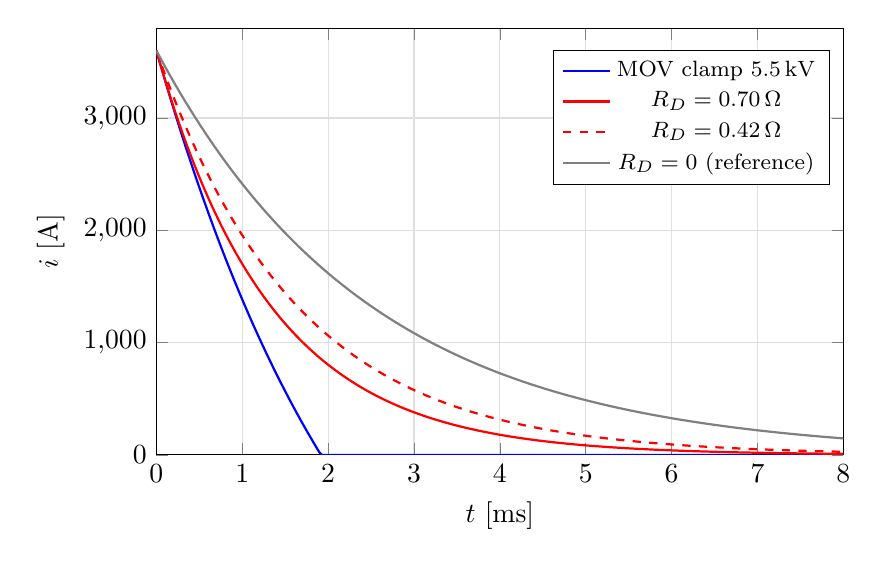
\begin{tikzpicture}
\begin{axis}[
  width=0.85\textwidth, height=7cm,
  xlabel={$t$ [\si{\milli\second}]},
  ylabel={$i$ [\si{\ampere}]},
  xmin=0, xmax=8, ymin=0, ymax=3800,
  grid=both, grid style={gray!25},
  legend style={font=\footnotesize, at={(0.98,0.95)}, anchor=north east},
  domain=0:8, samples=300,
]
\addplot[thick, blue]  {max(0, -3125 + 6725*exp(-x/2.5))};
\addlegendentry{MOV clamp \SI{5.5}{\kilo\volt}}
\addplot[thick, red]   {3600*exp(-x/1.333)};
\addlegendentry{$R_D=\SI{0.70}{\ohm}$}
\addplot[thick, red, dashed] {3600*exp(-x/1.639)};
\addlegendentry{$R_D=\SI{0.42}{\ohm}$}
\addplot[thick, gray]  {3600*exp(-x/2.5)};
\addlegendentry{$R_D=0$ (reference)}
\end{axis}
\end{tikzpicture}
\caption{Current decay after switch turn-off. The MOV clamp reaches a hard
zero in \SI{1.9}{\milli\second}; the dump resistor gives an exponential decay
of comparable speed. With $R_D=\SI{0.42}{\ohm}$ the peak switch voltage stays
at \SI{4.5}{\kilo\volt}.}
\label{fig:decay}
\end{figure}

Two observations:
\begin{itemize}
\item With $R_D \approx \SI{0.7}{\ohm}$ the extinction speed is essentially
that of the MOV clamp (the current is below $5\%$ of $I_0$ after
\SI{4}{\milli\second}), the peak switch voltage is the same
\SI{5.5}{\kilo\volt} but only instantaneous, and the absorber energy per
operation drops from \SI{16.6}{\kilo\joule} in a degrading nonlinear
component to \SI{6.0}{\kilo\joule} in a linear metallic one.
\item With $R_D \approx \SI{0.42}{\ohm}$ the peak switch voltage falls to
\SI{4.5}{\kilo\volt}, i.e.\ back inside the region where the RBSOA of a
\SI{6.5}{\kilo\volt} HiPak is actually specified \cite{hipak,igbtapp}. The
dump resistor therefore solves the RBSOA overreach of the
\SI{5.5}{\kilo\volt} MOV clamp at the same time as the life problem, at the
cost of a moderately longer current tail.
\end{itemize}

\subsection{Reaching an actual current zero}

The exponential \eqref{eq:dumpdecay} never reaches zero mathematically; in
practice the crowbar thyristor turns off when the current falls below its
holding current $I_H$ (fractions of an ampere), at
$t \approx \tau_d \ln(I_0/I_H) \approx \SI{15}{\milli\second}$, which is a
true, arc-free current zero.

If the application requires a hard zero on the millisecond scale, a small
varistor of clamping voltage $V_M$ can be placed in series with $R_D$. The
loop equation becomes affine,
\begin{equation}
L\frac{di}{dt} = -(R_L+R_D)\,i - V_M ,
\end{equation}
with a finite extinction time
\begin{equation}
t_z = \tau_d \ln\!\left(1 + \frac{I_0 (R_L+R_D)}{V_M}\right).
\end{equation}
This option should be weighed carefully: the series varistor absorbs
$E_M = V_M Q$ with $Q$ of the order of \SI{3}{\coulomb}, i.e.\ several
kilojoules for $V_M$ in the kilovolt range --- it merely reintroduces the MOV
duty at reduced scale. It is preferable to accept the exponential tail and
the holding-current turn-off, unless the test specification explicitly
demands otherwise.

\section{Commutation into the dump branch}
\label{sec:commutation}

This is the one genuinely critical design detail of the scheme. The main
switch turns off in about a microsecond; the load current must therefore be
picked up by the crowbar branch at a rate that the crowbar device tolerates.
Two implementations are proposed.

\subsection{Option A: thyristor crowbar}
\label{sec:optA}

A single phase-control thyristor, e.g.\ the \SI{6.5}{\kilo\volt}
5STP~26N6500 \cite{pct}, comfortably provides the required ratings: reverse
blocking of $V_s = \SI{3}{\kilo\volt}$ with a factor-2 margin, surge capability
far above \SI{3600}{\ampere} for milliseconds, and natural turn-off at the
holding current. Points of attention:

\paragraph{Gating while reverse-biased.} Before the main switch opens, the
thyristor sits reverse-biased at $-V_s$ and cannot be fired. The gate must
be driven with a pulse train (with back porch) starting shortly before the
turn-off command, so that the device latches as soon as it becomes
forward-biased. Gate current applied under reverse bias increases the reverse
leakage and its dissipation; the arming lead time should therefore be kept
short (e.g.\ about \SI{100}{\micro\second}), which is trivial since the
interruption instant is commanded by the bench itself.

\paragraph{Turn-on $di/dt$.} A phase-control thyristor tolerates a repetitive
turn-on $di/dt$ of the order of \SIrange{100}{300}{\ampere\per\micro\second}
(data-sheet value to be respected at $10^6$ repetitions), whereas the raw
commutation would demand several \si{\kilo\ampere\per\micro\second}. A series
commutation inductance $L_c$ limits the rate. During the transfer the backup
MOV holds the switch at $V_c$, so the voltage driving the current into the
branch is $V_c - V_s \approx \SI{2.5}{\kilo\volt}$:
\begin{equation}
\left.\frac{di_{\mathrm{CB}}}{dt}\right|_{0} = \frac{V_c - V_s}{L_c},
\qquad L_c = \frac{\SI{2.5}{\kilo\volt}}{\SI{200}{\ampere\per\micro\second}}
\approx \SI{12.5}{\micro\henry},
\end{equation}
an inductance largely provided for free by a grid-type dump resistor and its
connections. The transfer completes in some tens of microseconds; during this
interval the MOV bank carries the difference current and absorbs
\begin{equation}
E_{\mathrm{MOV,comm}} \approx V_c \int (i_L - i_{\mathrm{CB}})\,dt
\approx \SIrange{200}{350}{\joule}
\end{equation}
per operation (the exact value depends on $R_D$ and $L_c$; with
$R_D=\SI{0.42}{\ohm}$, $L_c=\SI{12.5}{\micro\henry}$ the transfer takes
$\approx\SI{28}{\micro\second}$ and the MOV absorbs $\approx\SI{230}{\joule}$).
Spread over the bank this is \SIrange{15}{25}{\joule} per disc per operation,
i.e.\ about $2\%$ of the single-pulse class: a level that the repetitive
derating curves of block varistors may admit at $10^6$ pulses, \emph{to be
verified on the data-sheet derating chart} \cite{siov}. A saturable
commutation reactor (high unsaturated inductance for the first microseconds,
then saturating) reduces this residual MOV duty further, a standard technique
in pulse-power circuits.

\paragraph{Re-applied voltage.} After extinction the branch sees no voltage
(the switch is open); reverse voltage returns only at the next closing of the
main switch, many seconds later, so the circuit-commutated recovery time
$t_q$ is irrelevant. An RC snubber across the thyristor handles the
re-applied $dv/dt$ at switch closing.

\subsection{Option B: pre-triggered IGBT crowbar}
\label{sec:optB}

The crowbar can instead be an IGBT (or two paralleled modules of the same
5SNA~1000G650300 family) in series with a blocking diode oriented to conduct
from the return rail into node~A. During normal operation the diode blocks
$V_s$; the crowbar IGBT can simply be held \emph{on} for the whole armed
period. At main-switch turn-off the branch picks up the current with no
firing delay and no $di/dt$ limitation other than the loop stray inductance:
the residual MOV duty of Option~A essentially disappears.

Ratings: with two paralleled modules each carries \SI{1800}{\ampere} peak,
inside the \SI{1}{\milli\second} pulsed collector current rating
$I_{CM}=\SI{2000}{\ampere}$, and decaying. The conducted charge is
$Q = I_0 \tau_d \approx \SI{6}{\coulomb}$, so the conduction energy per
operation is $\sim V_{CE(\mathrm{sat})} Q \approx \SI{15}{\joule}$ ---
thermally negligible, with junction temperature excursions below
\SI{1}{\kelvin} per shot and therefore no power-cycling concern. The cost is
one more gate driver, one blocking diode under \SI{3}{\kilo\volt} DC (same
cosmic-ray considerations as the main switch \cite{voltrat}), and two more
modules.

Option~A is simpler and more rugged; Option~B is cleaner electrically. Both
are compatible with the life target.

\section{Dump resistor design}
\label{sec:resistor}

\paragraph{Energy and temperature per pulse.} With
$E_D=\SIrange{4.5}{6.0}{\kilo\joule}$ per operation, an adiabatic element of
mass $m$ and specific heat $c$ rises by $\Delta T = E_D/(m c)$ per pulse.
A stainless-steel or FeCrAl grid element of \SI{20}{\kilogram}
($c\approx\SI{480}{\joule\per\kilogram\per\kelvin}$) rises by only about
\SI{0.6}{\kelvin} per pulse: thermal fatigue is a non-issue.

\paragraph{Average power.} The average dissipation is $\bar P = E_D/T_{cyc}$:
\SI{100}{\watt} at one operation per minute, \SI{600}{\watt} at one per ten
seconds --- trivially handled by natural or light forced convection. The
cycle period of the bench should be confirmed, as it sets this number (and it
is the same number that would drive the MOV bank into thermal runaway).

\paragraph{Technology.} Grid or ribbon resistors of the braking-resistor
class are the natural choice: metallic conduction, no drift mechanism, low
temperature coefficient, and a parasitic inductance of a few microhenries
that is actually \emph{useful} in Option~A (it forms part of $L_c$). For
Option~B a lower-inductance construction (Ayrton--Perry or bifilar winding)
is preferable, with the residual $L_R\, di/dt$ overshoot at commutation
covered by the module snubbers and the backup MOV.

\paragraph{Life.} The cumulative energy over $10^6$ operations is
$\sim\SI{6}{\giga\joule}$ --- meaningless for a metallic element sized as
above, whereas the equivalent cumulative charge of $\sim\SI{3}{\mega\coulomb}$
through the MOV bank is far beyond any varistor capability. This asymmetry is
the core argument for the scheme.

\section{Residual role of the MOV bank}
\label{sec:backup}

The MOV bank is retained across the switch, but demoted from per-cycle
absorber to \emph{backup clamp}. Its duties become:
\begin{enumerate}
\item clamping the first microseconds of each commutation (Option~A only,
\SIrange{200}{350}{\joule} per operation, to be verified against the
repetitive derating curve, or reduced with a saturable reactor);
\item absorbing the full \SI{16.6}{\kilo\joule} event if the crowbar fails to
fire. The existing $3\mathrm{s}\times 5\mathrm{p}$ B80K680 bank is already
sized for this as a single event; the data-sheet surge count at this level
(tens of pulses) becomes an acceptable \emph{fault budget} rather than a
life-limiting consumable.
\end{enumerate}
Practical measures: count crowbar misfires (a misfire is directly observable
from the switch-voltage waveform), periodically verify
$V_{\SI{1}{\milli\ampere}}$ of the strings, and alarm on drift. A crowbar
device failed short is also benign and observable: it appears as a resistive
divider across the load at the next switch closing.

\section{Conclusions}

\begin{itemize}
\item The baseline MOV clamp absorbs $\approx\SI{16.6}{\kilo\joule}$ per
operation --- more than the stored inductive energy, because the source keeps
feeding the clamped loop. No varistor technology sustains this duty for
$10^6$ cycles; drift, parallel-string imbalance and average-power thermal
runaway all point the same way.
\item A dump resistor switched across the load by a crowbar extracts the
energy with the source disconnected: only $\tfrac{1}{2}LI_0^2$ is dissipated,
split between load and dump resistors, in components with practically
unlimited electrical life.
\item Extinction speed is preserved: with $R_D=\SI{0.7}{\ohm}$ the decay is
as fast as the MOV clamp; with $R_D=\SI{0.42}{\ohm}$ the peak switch voltage
drops to \SI{4.5}{\kilo\volt}, restoring margin to the specified RBSOA of the
\SI{6.5}{\kilo\volt} modules.
\item The critical implementation detail is the commutation $di/dt$: solved
with a \SIrange{10}{15}{\micro\henry} commutation inductance (thyristor
crowbar, Option~A) or eliminated with a pre-triggered IGBT + blocking diode
branch (Option~B).
\item The MOV bank remains as a backup clamp with a fault budget of tens of
full events, plus (Option~A) a small per-cycle commutation duty to be checked
against the repetitive derating curves.
\end{itemize}

\begin{thebibliography}{9}

\bibitem{mohan}
N.~Mohan, T.~M. Undeland, W.~P. Robbins,
\emph{Power Electronics: Converters, Applications, and Design},
3rd ed., Wiley, 2003.

\bibitem{greenwood}
A.~Greenwood,
\emph{Electrical Transients in Power Systems},
2nd ed., Wiley, 1991.

\bibitem{siov}
TDK Electronics,
\emph{SIOV Metal Oxide Varistors --- General Technical Information},
data book, 2018.

\bibitem{lhc}
K.~Dahlerup-Petersen \emph{et al.},
``Energy extraction in the CERN LHC: a project overview,''
in \emph{Proc.\ 13th IEEE Int.\ Pulsed Power Conference},
Las Vegas, NV, 2001.

\bibitem{hipak}
Hitachi Energy (formerly ABB Semiconductors),
\emph{5SNA 1000G650300 HiPak IGBT Module},
data sheet.

\bibitem{pct}
Hitachi Energy (formerly ABB Semiconductors),
\emph{5STP 26N6500 Phase Control Thyristor},
data sheet.

\bibitem{igbtapp}
ABB Switzerland Ltd.\ Semiconductors,
\emph{Applying IGBTs},
Application Note 5SYA 2053.

\bibitem{voltrat}
ABB Switzerland Ltd.\ Semiconductors,
\emph{Voltage Ratings of High Power Semiconductors},
Application Note 5SYA 2051.

\end{thebibliography}

\end{document}
